% \documentclass[onecolumn]{IEEEtran}
\documentclass[a4paper]{article}

\usepackage[utf8]{inputenc}
\usepackage{lmodern}
\usepackage[T1]{fontenc}
\usepackage[catalan]{babel}
\usepackage{mathtools}
\usepackage{upgreek}
\usepackage{float}
\usepackage{csvsimple}
\providecommand{\abs}[1]{\lvert#1\rvert}

% \usepackage[backend=biber,style=phys]{biblatex}
% \addbibresource{.bib}

% \usepackage{multirow}
\usepackage{multicol}
\usepackage{multirow}
\usepackage[table,xcdraw]{xcolor}
\usepackage{hhline}
\usepackage{rotating}
\usepackage{tikz}
\usepackage{graphicx}
\usepackage{wrapfig}
\usepackage{caption}
% \usepackage{subcaption}
% \usepackage{geometry}
% \geometry{
% a4paper,
% total={150mm,257mm},
% left=30mm,
% top=20mm,
% }
% \usepackage{graphicx}
% \usepackage{caption}
% \usepackage{subcaption}

\usepackage[a4paper]{geometry}
\geometry{top=2cm, bottom=3.3cm, left=2.5cm, right=2.5cm}
\usepackage{titling}
% \renewcommand{\arraystretch}{1.8} 
% \newcolumntype{M}{X<{\vspace{4pt}}} 
\usepackage{gensymb} %to use degrees
\usepackage{fancyhdr}
\usepackage[hidelinks]{hyperref}
\pagestyle{fancy}

\usepackage{braket}


\lhead{\bf MQDNCISU}
\rhead{Iris Ortega i Ferran Rodríguez}
\title{Entrega: Weakly interacting and confined bosons at low density}
\author{Iris Ortega i Ferran Rodríguez}


\begin{document}
\maketitle{}


% \subsection*{Enunciat}


% \textbf{The theoretical description of the recent experiments on Bose Einstein condensation (BEC) is based on the Gross-Pitaevskii (GP) equation. The atoms are confined by a magnetic field, which effects are very well described by an harmonic oscillator potential. Here we assume a condensate of $\boldsymbol{^{87}Rb}$. We made the assumption that all the atoms are in the condensate, $\boldsymbol{\Psi(\vec{r})}$ normalised such that:}
% \begin{equation}
%      \boldsymbol{\int d\vec{r}\ |\Psi(\vec{r})|^2=1 \ .}
% \end{equation}
% \textbf{In harmonic oscillator units, the GP equation reads:}
% \begin{equation}
%     \boldsymbol{\left[-\dfrac{1}{2}\nabla^2 +\dfrac{1}{2}r_1^2+4\pi \bar a_s N  |\bar\Psi(\vec{r}_1)|^2\right]\bar\Psi(\vec{r}_1)=\mu \bar\Psi(\vec{r}_1)\ ,}
% \end{equation}
% \textbf{where $\boldsymbol{\mu}$ is the chemical potential, $\mathbf{N}$ the number of particles and $\mathbf{a_s}$ the $\mathbf{s}$-wave scattering length in harmonic oscillator units. In this case, $\boldsymbol{\bar\Psi(\vec{r}_1)}$ is normalised to $\mathbf{1}$.}\\


\section{\bf Introducció}


Per fer l'exercici s'ha escrit un nou programa amb \textit{Python} i les llibreries \texttt{math}, \texttt{argparse}, \texttt{numpy} i \texttt{pandas}. L'hem anomenat \texttt{Iris\_Ortega-Ferran\_Rodriguez.py}\footnote{El programa ha estat escrit per l'Iris, les dades han sigut representades pel Ferran. La redacció s'ha fet entre els dos.}. Tots els resultats exposats en aquest treball obtinguts amb aquest programa, han estat comprovats amb els obtinguts amb el programa de \textit{Fortran} proporcionat. Per saber com funciona el nou programa es pot introduir al terminal:
\begin{quote}
    \texttt{python3 Iris\_Ortega-Ferran\_Rodriguez.py -h}.
\end{quote}
Per usar-lo només requereix un argument, el \textit{path} on es troba el fitxer \textit{input}, un fitxer \textit{.txt} amb tantes files com diferents valors de les variables es vulguin introduir i amb columnes corresponents a: la longitud de \textit{scattering} en unitats d'osci"lador (\texttt{a0}), el nombre de passes (\texttt{N\_steps}), la mida del pas (\texttt{step}), el nombre de partícules (\texttt{N}), el pas en el 'temps' (\texttt{time}), el valor d'alfa (paràmetre d'inici per la funció de l'osci"lador harmònic, \texttt{alpha}) i el nombre d'iteracions (\texttt{iter}). Afegint \texttt{-ao} obtenim el cas de l'osci"lador harmònic, mentre que afegint \texttt{-tf}, obtenim els resultats per l'aproximació de Thomas-Fermi.




% \subsubsection*{a0) Using the GP program check that if you put the interaction equal to zero, then you recover the expected results
% for the harmonic oscillator. Why is the energy per particle equal to the chemical potential?}


\section{\bf Interacció nu"la: solució per l'osci"lador harmònic}


En el nostre programa, per tenir la solució per l'osci"lador harmònic només cal afegir un darrer argument en la terminal: \texttt{-ao}. Això fa que la variable \texttt{cequ} del programa passi a valer $0$.

En córrer el programa per un \textit{input} tal com el de la Taula \ref{tab:input_a0}, obtenim $E=1.4999665803921967$ per l'energia i $\mu=1.4999665800446846$ pel potencial químic, ambdós en unitats de l'osci"lador harmònic. La diferència entre ambdós valors és de $10$ ordres de magnitud inferior a aquests: $E-\mu=3\cdot10^{-10}$. Per tant, tenim $E\approx \mu\approx 1.5$. 

\begin{table}[H]
    \centering
    \begin{tabular}{|c|c|c|c|c|c|c|}
    \hline
    \rowcolor[HTML]{EFEFEF}
       \textbf{\texttt{a0}} & \textbf{\texttt{N\_steps}} & \textbf{\texttt{step}} &\textbf{\texttt{N}} & \textbf{\texttt{time}} & \textbf{\texttt{alpha}} & \textbf{\texttt{iter}} \\ \hline\hline
       $0.00433$ & $700$ & $0.015$ & $1000000$ & $0.00005$ & $0.3$ & $70000$ \\ \hline
    \end{tabular}
\caption{\textit{Input} del programa per l'apartat a0).}
\label{tab:input_a0}
\end{table}

Les dues magnituds valen aproximadament el mateix, ja que en treure el terme corresponent a la interacció, l'equació de Gross-Pitaevski adimensional es redueix a una equació de Schrödinger adimensional per un potencial donat. Els autovalors resultats de l'equació de Schrödinger són les possibles energies del sistema, mentre que els de l'equació de Gross-Pitaevskii són els del potencial químic. Com que la part de l'esquerra d'ambdues equacions s'iguala, el resultat que obtenim per la dreta, els autovalors, és aproximadament el mateix.

% \subsubsection*{a) Take $\mathbf{\bar a_s = 0.0043}$, appropriate for $\mathbf{^{87}Rb}$ and, using the program, solve the Gross-Pitaevskii equation. Study the dependence on the number of particles ($\mathbf{N}=100, 1000, 10000, 100000, 1000000$) of the chemical potential, and the following energies per particle: total, kinetic, harmonic oscillator and interaction energy. Construct a table with the results and comment their behaviour.}


\section{\bf Solució de l'equació de Gross-Pitaevskii: dependència en $\boldsymbol{N}$}


Per trobar les solucions a l'equació de Gross-Pitaevskii hem usat com a \textit{input} el proporcionat en el fitxer \textit{grosspita.grau.input.txt}, que es troba recollit en la Taula \ref{tab:input_a}. Els resultats es troben a la Taula \ref{tab:res_a}.

\begin{table}[H]
    \centering
    \begin{tabular}{|c|c|c|c|c|c|c|}
        \hline
        \rowcolor[HTML]{EFEFEF}
        \textbf{\textit{a0}} & \textbf{\textit{N\_steps}} & \textbf{\textit{step}} &\textbf{\textit{N}} & \textbf{\textit{time}} & \textbf{\textit{alpha}} & \textbf{\textit{iter}} \\ \hline\hline
        0.00433 & 700 & 0.015 & 1000000 & 0.00005 & 0.3 & 70000 \\ \hline
        0.00433 & 600 & 0.015 & 100000  & 0.0001  & 0.4 & 50000 \\ \hline
        0.00433 & 400 & 0.015 & 10000   & 0.0001  & 0.8 & 40000 \\ \hline
        0.00433 & 400 & 0.020 & 1000    & 0.0001  & 0.5 & 50000 \\ \hline
        0.00433 & 300 & 0.020 & 100     & 0.0001  & 0.5 & 50000 \\ \hline
    \end{tabular}
\caption{\textit{Input} del programa per l'apartat a), corresponent al fitxer \textit{grosspita.grau.input.txt}.}
\label{tab:input_a}
\end{table}

\begin{table}[]
\centering
\begin{tabular}{|c|c|c|c|c|c|c|}
\hline
    \rowcolor[HTML]{EFEFEF}
    $\mathbf{N}$ & $\boldsymbol{\mu}$ & $\boldsymbol{\mu_{\textbf{T}}}$ & $\boldsymbol{E_{\textbf{T}}}$ & $\boldsymbol{E_{\textbf{cin.}}}$ & $\boldsymbol{E_{\textbf{osc.}}}$ & $\boldsymbol{\mu_{\textbf{inter.}}}$ \\ \hline\hline
    \textbf{1000000}  & 42.119 & 30.059  & 30.120     & 0.061  & 18.060 & 11.999   \\ \hline
    \textbf{100000}   & 16.847 & 11.980  & 12.104     & 0.124  & 7.238  & 4.743    \\ \hline
    \textbf{10000}    & 6.866  & 4.801   & 5.042      & 0.240  & 2.977  & 1.824    \\ \hline
    \textbf{1000}     & 3.045  & 1.987   & 2.425      & 0.438  & 1.367  & 0.620    \\ \hline
    \textbf{100}      & 1.788  & 0.995   & 1.652      & 0.656  & 0.860  & 0.136    \\\hline
\end{tabular} 
    \caption{Resultats d'introduir al programa l'\textit{input} de la Taula \ref{tab:input_a}. Per cada nombre de partícules al sistema tenim el potencial químic mitjà corresponent, el total, l'energia total, la cinètica, la corresponent a l'osci"lador harmònic i la corresponent al terme d'interacció. S'observa que el potencial total equival a la suma del corresponent a l'osci"lador harmònic més el del terme d'interacció mentre que l'energia total és el potencial total més l'energia corresponent al terme cinètic.}
    \label{tab:res_a}
\end{table}

\begin{figure}[H]
    \centering
    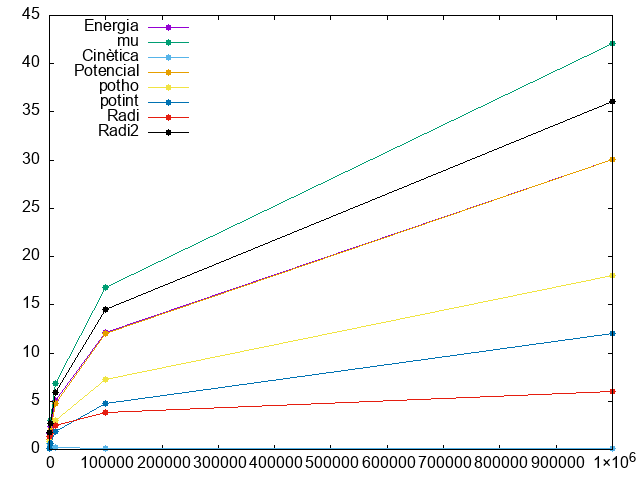
\includegraphics[width=0.7\linewidth]{../a.png}
\caption{Representació doble logarítmica de les dades recollides a la Taula~\ref{tab:res_a}.}
\label{fig:res_a}
\end{figure}

Observem com a la Fig.~\ref{fig:res_a} l'energia i el moment totals augmenten segons $N$, amb la mateixa força amb què ho fan les diferents components d'aquestes, exceptuant l'energia cinètica, que sembla que disminueixi amb el comportament oposat a les altres components.

Com més partícules hi hagi, més difícil en serà extreure'n una del sistema. Per això el potencial químic i les diferents energies (menys la cinètica) augmenten. L'energia cinètica disminueix amb el nombre de partícules perquè aquestes xocaran més i perdran més energia.

Veiem com, en al representació doble logarítmica, es tendeix a un comportament lineal per $N$ grans, presentant desviacions significatives per $N < 10^3-10^4$.

El potencial i l'energia totals tendeixen a igualar-se per $N$ grans.


% \subsubsection*{b) Do the same using the Thomas-Fermi approximation. Notice that the kinetic energy in this approach is taken to zero.}


\section{\bf Aproximació de Thomas-Fermi}


\begin{table}[H]
\centering
\begin{tabular}{|c|c|c|c|c|c|}
\hline
    \rowcolor[HTML]{EFEFEF}
    $\mathbf{N}$ & $\boldsymbol{\mu}$ & $\boldsymbol{\mu_{\textbf{T}}}$ & $\boldsymbol{E_{\textbf{T}}}$ & $\boldsymbol{E_{\textbf{osc.}}}$ & $\boldsymbol{\mu_{\textbf{inter.}}}$ \\ \hline\hline
    \textbf{1000000}   & 42.071 & 30.052  & 30.052 & 18.033 & 12.019   \\ \hline
    \textbf{100000}    & 16.748 & 11.964  & 11.964 & 7.180  & 4.784    \\ \hline
    \textbf{10000}     & 6.670  & 4.763   & 4.763  & 2.856  & 1.907    \\ \hline
    \textbf{1000}      & 2.647  & 1.897   & 1.897  & 1.147  & 0.750    \\ \hline
    \textbf{100}       & 1.045  & 0.759   & 0.759  & 0.472  & 0.286    \\ \hline
\end{tabular}
    \caption{Resultats d'introduir al programa l'\textit{input} de la Taula \ref{tab:input_a} i còrrer el programa usant l'aproximació de Thomas-Fermi (afegint \texttt{-tf} a la línia de comandes). Per cada nombre de partícules al sistema tenim el potencial químic mitjà corresponent, l'energia total, la corresponent a l'osci"lador harmònic i la corresponent al terme d'interacció. Observem que en aquest cas, el potencial total i l'energia total són equivalents.}
    \label{tab:res_b}
\end{table}

\begin{figure}[H]
    \centering
    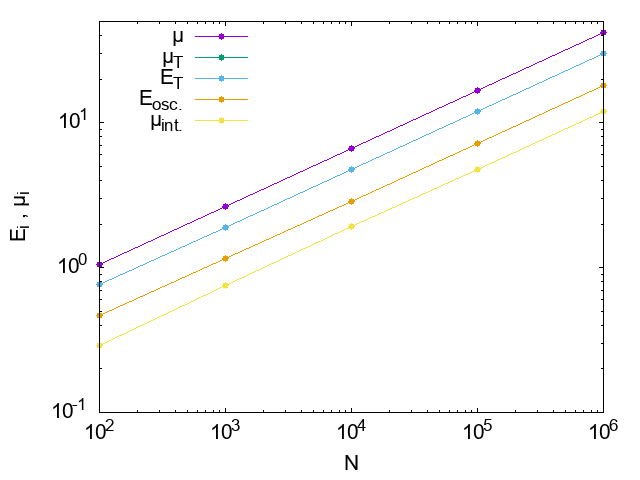
\includegraphics[width=0.7\linewidth]{../b.png}
\caption{Representació doble logarítmica de les dades recollides a la Taula~\ref{tab:res_b}. Els valors per a $\mu_T$ i $E_T$ són iguals.}
\label{fig:res_b}
\end{figure}

Els resultats per a l'aproximació de Thomas-Fermi s'assemblen més als de l'apartat anterior com més gran és $N$, ja que l'energia cinètica disminueix quan s'augmenta $N$.

Si fem la regressió lineal de les dades de l'energia total de la Fig.~\ref{fig:res_b}, obtenim que $E_T = 0.12 N^{0.40}$, amb un error dels coeficients molts ordres de magnitud inferior. Per tant, veiem que les diferents energies i potencials tenen una dependència amb el nombre de partícules de $\sim N^{2/5}$, que en l'aproximació de Thomas-Fermi es compleix per tot el rang de $N$ mentre que quan tenim energia cinètica veiem desviació a $N$ baixes, com és d'esperar.


% \subsubsection*{c) Make a plot of the density profile $\boldsymbol{\rho (r_1)}$ normalised such that \begin{equation}
%     \boldsymbol{\int dr_1  r_1^2 \rho(r_1)=1}
% \end{equation} for $\mathbf{N=1000}$ and $\mathbf{N=100000}$ and compare the GP and the TF results.}


\section{\bf Perfil de la densitat}


\begin{figure}[H]
    \centering
    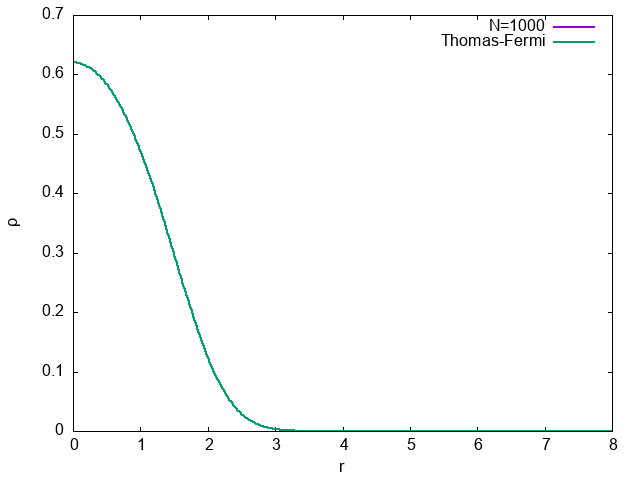
\includegraphics[width=0.49\linewidth]{../c1000.png}
    % \caption{Representació del perfil de densitat normalitzat amb $N=1000$ pel cas sense aplicar i aplicant l'aproximació de Thomas-Fermi.}
    % \label{fig:res_c1000}
    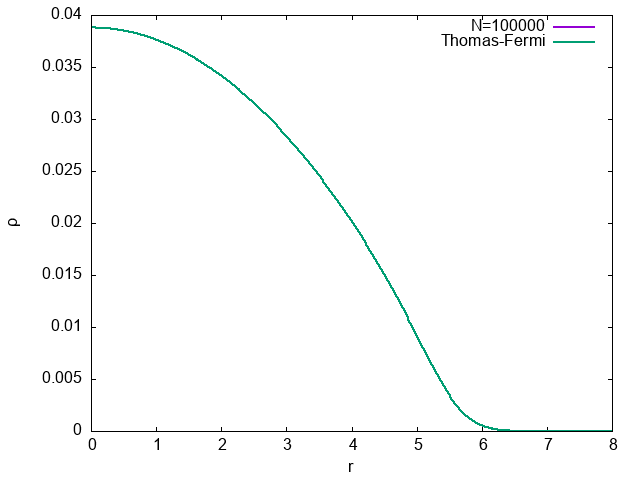
\includegraphics[width=0.49\linewidth]{../c100000.png}
    \caption{Representació del perfil de densitat normalitzat amb $N=1000$ (esquerra) i $N=100000$ (dreta), comparant el cas sense aplicar amb el cas en què s'aplica l'aproximació de Thomas-Fermi.}
    \label{fig:res_c}
\end{figure}

Com ja comentàvem en la secció anterior, l'aproximació de Thomas-Fermi s'ajusta millor per $N$ grans, tal i com es pot veure altre cop en la Fig. \ref{fig:res_c}.


% \subsubsection*{d) Check numerically that the solutions of the GP equation fulfill the virial theorem for different values of $\mathbf{N}$.}


\section{\bf Comprovació numèrica del teorema del virial}


Per trobar l'equació corresponent al teorema del Virial ens construïm la funció $\Psi_{\lambda}(\{\vec r'\})=\lambda^{3N/2}\Psi_{\text{G.S}}(\{\lambda\vec r\})$, on G.S. vol dir \textit{ground state}. Aleshores, calculem l'autovalor de l'equació de GP:
\begin{equation}
   \langle E(\lambda)\rangle=\int d^{3N}\vec r \ \Psi_{\lambda}^{*}(\{\vec r'\})\mathcal{H} \Psi_{\lambda}(\{\vec r'\}) \ .
\end{equation}
Fent el canvi de variable $\vec r\ '= \lambda\vec r$, obtenim per partícula: 
\begin{equation}
    \nabla^2_{\vec r}=\lambda^2\nabla^2_{\vec r\ '}, \quad \vec r^2=\dfrac{{\vec r}^{\ '2}}{\lambda^2}, \quad |\Psi_{\lambda}(\{\vec r\ '\})|^2=\lambda^3\Psi_{G.S.}|(\{\vec r\ '\})|^2 \ .
\end{equation}
Substituint aquests valors obtenim:
\begin{equation}
    e= \lambda^2 e_{\text{cin.}}+\dfrac{1}{\lambda^2}e_{\text{osc.}}+\lambda^3 e_{\text{int.}}\ .
\end{equation}
I imposant condició d'extrem obtenim l'equació del Virial:
\begin{equation}
    \left.\dfrac{de(\lambda)}{d\lambda}\right\vert_{\lambda=1}=2e_{\text{cin.}}-2e_{\text{osc.}}+3 e_{\text{int.}}=0\ .
    \label{eq:Virial}
\end{equation}
Aleshores, aplicant l'Eq. \ref{eq:Virial} pels resultats de la Taula \ref{tab:res_a}, obtenim els valors de la Taula \ref{tab:res_d}.
\begin{table}[H]
\centering
\begin{tabular}{|c|c|}
\hline
\rowcolor[HTML]{EFEFEF}
\textbf{N} & $\mathbf{2e_{\text{cin.}}-2e_{\text{osc.}}+3 e_{\text{int.}}}$ \\ \hline\hline
\textbf{1000000}  & $4\cdot10^{-4}$      \\ \hline
\textbf{100000}   & $5\cdot10^{-6}$     \\ \hline
\textbf{10000}    & $2\cdot10^{-5}$     \\ \hline
\textbf{1000}     & $4\cdot10^{-5}$     \\ \hline
\textbf{100}      & $4\cdot10^{-5}$     \\ \hline
\end{tabular}
\caption{Resultats de fer la suma del teorema del Virial corresponent a la nostra equació de GP per diferents valors de $N$ amb les dades recollides en la Taula \ref{tab:res_a}. S'han aproximat al primer valor diferent de $0$ per saber els ordres de magnitud de diferència respecte al resultat del teorema del Virial.}
\label{tab:res_d}
\end{table}

Observem que els resultats difereixen del $0$ del teorema del Virial en $4$ fins a $6$ ordres de magnitud. Per tant, considerem que el teorema es compleix.

\end{document}